\documentclass[a4paper,12pt]{article} 
\usepackage[top = 2.5cm, bottom = 2.5cm, left = 2.5cm, right = 2.5cm]{geometry} 

\usepackage[T1]{fontenc}
\usepackage[utf8]{inputenc}
\usepackage{amsmath}
\usepackage{amssymb}
\usepackage{halloweenmath}
\usepackage{lipsum}

\usepackage{multirow} 
\usepackage{booktabs}
\usepackage{graphicx} 

\usepackage{setspace}
\setlength{\parindent}{0in}

\usepackage{float}

\usepackage{fancyhdr}
\usepackage[colorlinks=true,linkcolor=blue]{hyperref}
\usepackage{amsmath}
\usepackage{tikz}
\usetikzlibrary{tikzmark}

%%%%%%%%%%%%%%%%%%%%%%%%%%%%%%%%%%%%%%%%%%%%%%%%
% 3. Header (and Footer)
%%%%%%%%%%%%%%%%%%%%%%%%%%%%%%%%%%%%%%%%%%%%%%%%
\pagestyle{fancy} 
\fancyhf{} 
\lhead{\footnotesize }
\footnotesize 
\rhead{\footnotesize Collins \thepage} 
\cfoot{\footnotesize} 


%%%%%%%%%%%%%%%%%%%%%%%%%%%%%%%%%%%%%%%%%%%%%%%%
% 4. Your document
%%%%%%%%%%%%%%%%%%%%%%%%%%%%%%%%%%%%%%%%%%%%%%%%
\begin{document}

%%%%%%%%%%%%%%%%%%%%%%%%%%%%%%%%%%%%%%%%%%%%%%%%
% Title section of the document
%%%%%%%%%%%%%%%%%%%%%%%%%%%%%%%%%%%%%%%%%%%%%%%%
\thispagestyle{empty} 

\begin{tabular}{p{15.5cm}} 
\\ Collin Collins \\
MATH 3400\\
SI Session 11 Final Exam Review\\
20 April 2024 \\
\hline 
\\
\end{tabular}


\subsection*{Problem 1} Suppose a 100 L, well-stirred tank contains 10 L of pure water. At some point, a feed of 2 L/min is started which contains 1 kg/L of salt. The tank begins to drain at a rate of 1 L/min. How much salt is in the tank when the tank is full?
\\
 
Try it out before looking at the solution.
\pagebreak

\textbf{Solution to Problem 1:}\\
Let's make a list of our knowns:

$$\left\{\begin{array}{ll}V_o=10 & Q_o=0 \\ V_{\text {max }}=100 & V(t)=t+10 \\ r_{\text {in }}=2 & r_{\text {out }}=1 \\ c_{\text {in }}=1 & c_{\text {out }}=\frac{Q(t)}{t+10}\end{array}\right\}$$
Using the following definition:
$$ \frac{dQ}{dt} \triangleq r_{\text{in}}c_{\text{in}} - r_{\text{out}}c_{\text{out}},$$
we have:
$$ \frac{dQ}{dt} = (2)(1) - (1)\left(\frac{Q(t)}{t+10}\right). $$
Rearranging:
$$ Q' + \underbrace{\frac{1}{t+10}}_{p(t)}Q = \underbrace{2}_{f(t)}. $$
This is a F.O.L. differential equation, so we use the following key to its solution:
$$ \mu Q = \int \mu f dt. $$
We first find $\mu$, using the following definition:
$$ \mu \triangleq e^{\int pdt}. $$
With our value for $p(t)$:
$$ \mu = e^{\int \frac{1}{t+10}dt} \quad\implies\quad \mu = e^{\ln{|t+10|}} \quad\implies\quad \mu = (t+10). $$
With $\mu$ and $f$, we can find the RHS of the key to F.O.L. by evaluating the integral:
$$ \int \mu f dt = \int (t+10)(2)dt \quad\implies\quad \text{RHS} = 2\left[\frac{t^2}{2} + 10t + C\right] \quad\implies\quad \text{RHS} = t^2 + 20t + C_2. $$
Now, let's put things together:
$$ \mu Q = \text{RHS} \quad\implies\quad \mu Q = t^2 + 20t + C_2 \quad\implies\quad Q_g = \frac{t^2 + 20t + C_2}{t + 10}. $$
Since we have the initial condition that $Q(0)=0$, we can find the specific solution for the amount of salt as a function of time:
$$ Q(0)=0 \quad\therefore\quad 0 = \frac{0^2 + 20(0) + C_2}{10} \quad\implies\quad C_2 = 0-0-0 \quad\implies\quad C_2 = 0. $$
Our specific solution is:
$$ \boxed{Q_s(t) = \frac{t^2 + 20t}{t + 10}} $$
We aren't done quite yet. Let's find the amount of time it takes for the tank to fill with our solution:
$$ V(t^{\star}) = V_{\text{max}} \quad\therefore\quad V_{\text{max}} = t^{\star} + 10 \quad\implies\quad 100 = t^{\star} + 10  \quad\implies\quad t^{\star} = 90{\text{ min}}.$$
To find the amount of salt at this time, let's plug this value into our specific solution:
$$ Q_{s}(90) = \frac{(90)^2 + 20(90)}{90 +10} \quad\implies\quad \underline{\boxed{Q_s(90) = \frac{90^2 + 1800}{100} \text{ kg}}} $$

\pagebreak

\subsection*{Problem 2:} Solve the following IVP:

$$ yy' = 2y^2 + x \quad;\quad y(0  )=-1. $$

 
Try it out before looking at the solution.
\pagebreak

\textbf{Solution to Problem 2:}

With this problem, we start off by identifying the differential equation type. Since this is first order, let's see if it is first order linear:
$$ y' = 2y + \frac{x}{y} \quad\implies\quad y' - 2y = x y^{-1}.$$
It is almost F.O.L. save for the power of $y$ being multiplied to our function of $x$ on the RHS. This appears to be a Bernoulli's equation where $n=-1$.\\

The substitution factor in this case is $v=y^{1-n}$, so for our problem, we have:
$$ v=y^{1-(-1)} \quad\implies\quad \boxed{v=y^{2}} $$
Taking the implicit derivative of $v$:
$$ v' = 2yy' \quad\implies\quad \boxed{y' = \frac{v'}{2y}} $$
Let's make this substitution:
$$ \frac{v'}{2y} - 2y = \frac{x}{y}. $$
Multiplying everything by $2y$ to make our leading derivative monic, we have:
$$ v' - 4y^2 = 2x. $$
Noticing that $y^2 = v$ and making the substitution, we have:
$$ v' \underbrace{- 4}_{p(x)}v = \underbrace{2x}_{f(x)}. $$
This is a F.O.L. differential equation. It's solution is found with:
$$ \mu v = \int \mu f dx. $$
Finding $\mu$:
$$ \mu \triangleq e^{\int p dx} \quad\implies\quad \mu = e^{-4\int dx} \quad\implies\quad \mu = e^{-4x}. $$
Evaluating the RHS of the solution key:
$$ \text{RHS} = \int e^{-4x}(2x)dx \quad\implies\quad \text{RHS} = 2\int x e^{-4x}dx \quad \left\{ \begin{matrix}
	u = x & dv = e^{-4x} dx \\
	du = dx & v = -\frac{1}{4}e^{-4x}
\end{matrix}\right\} \quad\implies\ldots
$$
$$ \ldots\implies\quad \text{RHS} =  2\left[-\frac{xe^{-4x}}{4} + \frac{1}{4} \int e^{-4x}dx \right] \quad\implies\quad \text{RHS} = 2\left[-\frac{xe^{-4}}{4} + \frac{1}{4}\left(-\frac{1}{4}e^{-4x} + C\right)\right]. $$
Distributing the factors of 2 and $\frac{1}{4}$:
$$ \mu v = -\frac{xe^{-4x}}{2} - \frac{e^{-4x}}{8} + C_2 \quad\overset{\text{divide by $\mu$}}\implies\quad v = -\frac{x}{2} - \frac{1}{8} + C_2e^{4x}. $$
Replacing $v$ with $y^2$:
$$ y^2 = -\frac{x}{2} - \frac{1}{8} + C_2e^{4x} \quad\implies\quad \boxed{y_g = \sqrt{-\frac{x}{2} - \frac{1}{8} + C_2e^{4x}}} $$
Let's use our initial condition to find the specific solution:
$$ y(0)=-1 \quad\therefore\quad -1 = \sqrt{-\frac{(0)}{2} - \frac{1}{8} + C_2e^{4(0)}} \quad\implies\quad 1 = -\frac{1}{8} + C_2 \quad\implies\quad \boxed{C_2 = \frac{9}{8}} $$
Our specific solution will have a square root, leading us to think that there are positive and negative values of $y$ for any given value of $x$. This is not the case, our initial condition tells us that one of our values of $y$ is negative, meaning our solution is concerned with the negative half of the square root:
$$ \underline{\boxed{y_s = -\left|\sqrt{-\frac{x}{2} - \frac{1}{8} + \frac{9}{8}e^{4x}}\right|}} $$

\pagebreak

\subsection*{Problem 3} Solve the following IVP using the method of undetermined coefficients:

$$ y''-2y'+y=\sin(x) \quad;\quad y(0)=1 \quad;\quad y'(0)=1. $$

Try it out before looking at the solution.
\pagebreak

\textbf{Solution to Problem 3:}

With this solution technique, remember that our final solution will be the superposition of our complementary and particular solutions:
$$ y_g = y_c + y_p. $$

We start off by finding the solution for the homogenous case (the complementary solution):
$$ y'' -2y' + y = 0. $$
The discriminant is:
$$D \triangleq b^2 -4ac \quad\implies\quad D = (-2)^2 - 4(1)(1) \quad\implies\quad D = 4-4  \quad\implies\quad D=0.$$
This tells us that our complementary solution will have the form:
$$ y_c = C_1e^{\lambda x} + C_2xe^{\lambda x}. $$
Let's find our root:
$$ \lambda \triangleq \frac{-b \pm \sqrt{D}}{2a} \quad\implies\quad \lambda = \frac{2 \pm 0}{2} \quad\implies\quad \lambda = 1.$$
Our complementary solution is then:
$$ \boxed{y_c = C_1e^{x} + C_2xe^{x}}$$
To find our particular solution, we examine the form of the inhomogeneity, $\sin{(x)}$. We make the ansatz that our particular solution will be of the form:
$$ y_{p_{\text{guess}}} = A\sin{(x)} + B\cos{(x)}. $$
Taking the derivatives of our guess:
$$ y_{p_{\text{guess}}}' = A\cos{(x)} - B\sin{(x)}. $$
$$ y_{p_{\text{guess}}}'' = -A\sin{(x)} - B\cos{(x)}. $$
We plug these into our differential equation and determine the values of $A$ and $B$ that force a true statement:
$$ \big[-A\sin{(x)} - B\cos{(x)}\big] - 2\big[A\cos{(x)} - B\sin{(x)}\big] + \big[A\sin{(x)} + B\cos{(x)}\big] = \sin{(x)}. $$
Let's group terms by their function, making sure to distribute the 2:
$$ \big[-A + 2B + A\big]\sin{(x)} + \big[-B - 2A + B\big]\cos{(x)} = [1]\sin{(x)} + [0]\cos{(x)}. $$
The coefficients of the $\sin{(x)}$ on the LHS need to be equal to 1. The coefficients of the $\cos{(x)}$ on the LHS need to be equal to 0.
$$ -A + 2B + A = 1 \quad\implies\quad 2B = 1 \quad\implies\quad \boxed{B = \frac{1}{2}} $$
$$ -B - 2A + B = 0 \quad\implies\quad -2A = 0 \quad\implies\quad \boxed{A=0} $$
We have determined the coefficients, let's plug them into $y_{p_{\text{guess}}}$ to get our particular solution:
$$ \boxed{y_{p} = \frac{1}{2}\cos{(x)}} $$
Our general solution is then:
$$ \boxed{y_g = C_1e^x + C_2xe^x + \frac{1}{2}\cos{(x)}} $$
Using our first initial condition, $y(0)=1$:
$$ 1 = C_1 + 0 + \frac{1}{2} \quad\implies\quad C_1 = \frac{1}{2}. $$
Taking the derivative of our general solution so that we can use the second initial condition:
$$ y_g' = C_1e^x + C_2e^{x} + C_2xe^x - \frac{1}{2}\sin{(x)}. $$
Now, using the second initial condition, y'(0)=1:
$$ 1 = C_1 + C_2 + 0 - 0 \quad\implies\quad C_1 + C_2 = 1 \quad\implies\quad \frac{1}{2} + C_2 = 1 \quad\implies\quad C_2 = \frac{1}{2}. $$
Our final, specific solution is:
$$ \underline{\boxed{y_s(x) = \frac{1}{2}\big[e^x + xe^x + \cos{(x)}\big]}}$$

\pagebreak

\subsection*{Problem 4} Find the general solution using variation of parameters:

$$ y''-2y'+y=2e^{3t}. $$

Try it out before looking at the solution.
\pagebreak

\textbf{Solution to Problem 4:}

Using the variation of parameters technique will give us a general solution that has this form:
$$ y_g = \underbrace{y_c}_{C_1y_1 + C_2y_2} + \underbrace{y_p}_{\mu_1y_1 + \mu_2y_2} $$
Here, the complementary solution is found by solving the homogenous case of this differential equation. The particular solution is expressed above as: $\mu_1y_1 + \mu_2y_2$. Naturally, we want to find out what $\mu_1$ and $\mu_2$ are ($y_1$ and $y_2$ come from the complementary solution). 

$$ \mu_1 \triangleq -\int \frac{y_2 f}{W[y_1, y_2]} dt \quad\text{ and }\quad \mu_2 \triangleq \int \frac{y_1 f}{W[y_1, y_2]} dt. $$
Let's start off by finding the complementary solution.\\

Oop, it's just the same as the previous problem, so let's use that:
$$ y_c = C_1\underbrace{e^{t}}_{y_1} + C_2\underbrace{te^{t}}_{y_2}. $$
With $y_1$ and $y_2$, we can take the Wronskian:
$$ W[y_1, y_2] \triangleq \left|\begin{matrix}
	 y_1 & y_2 \\
	 y_1' & y_2'
\end{matrix}\right|. $$
For our values of $y_1$ and $y_2$:
$$ W[e^t, te^t] = \left|\begin{matrix}
	e^t & te^t \\
	e^t & (e^t + te^t)
\end{matrix} \right| \quad\implies\quad W = e^t(e^t + te^t) - e^t(te^t) \quad\implies\quad W = e^{2t} + te^{2t} - te^{2t} \quad ... $$
$$ \boxed{W = e^{2t}} $$
With the Wronskian, we can begin finding $\mu_1$ and $\mu_2$. Let's start with $\mu_1$.
$$ \mu_1 = -\int \frac{te^t2e^{3t}}{e^{2t}}dt \quad\implies\quad \mu_1 = -2\int\frac{te^{4t}}{e^{2t}}dt \quad\implies\quad \mu_1 = -2 \int te^{2t}dt\quad ...
$$
$$ \left\{\begin{matrix}
	u = t & dv = e^{2t}dt\\
	du = dt & v = \frac{1}{2}e^{2t}
\end{matrix}\right\} \quad\implies\quad \mu_1 = -2\left[\frac{te^{2t}}{2} - \int \frac{1}{2}e^{2t}dt\right] \quad\implies\quad \boxed{\mu_1 = -te^{2t} +\frac{1}{2}e^{2t}} $$
Now, we find $\mu_2$:
$$ \mu_2 = \int \frac{e^{t}2e^{3t}}{e^{2t}}dt \quad\implies\quad \mu_2 = 2\int \frac{e^{4t}}{e^{2t}}dt \quad\implies\quad \mu_2 = 2\int e^{2t}dt \quad\implies\quad \boxed{\mu_2 = e^{2t}} $$
Our particular solution is then:
$$ y_p = \mu_1y_1 + \mu_2y_2 \quad\implies\quad y_p = \left(\frac{1}{2}e^{2t} - te^{2t}\right)e^t + (e^{2t})te^{t} \quad\implies\quad y_p = \frac{1}{2}e^{3t} -te^{3t} + te^{3t} \quad... $$
$$ \boxed{y_p = \frac{1}{2}e^{3t}}  $$
Putting everything together to get our general solution:
$$ \underline{\boxed{y_g(t) = C_1e^t + C_2te^t + \frac{1}{2}e^{3t}}} $$

\pagebreak

\subsection*{Problem 5} Solve the following IVP using the Laplace method:

$$ y''+2y'+ y=\mu_0(t) \quad;\quad y(0)=0\quad;\quad y'(0)=0. $$

Try it out before looking at the solution.
\pagebreak

\textbf{Solution to Problem 5:}

I'll start off by giving you the Laplace transforms that were given on the first page of the exam that this problem was inspired by:

\begin{table}[ht!]
\begin{center}
\renewcommand{\arraystretch}{1.3}
\begin{tabular}{| c | c |}
\hline
$t^n$ & $\displaystyle\frac{n!}{s^{n+1}}$ \\
\hline
$e^{-at}f(t)$ & $F(s+a)$ \\
\hline
$\mu(t-a)f(t-a)$ & $e^{-as}F(s)$ \\
\hline
$\delta(t-a)$ & $e^{-as}$ \\
\hline
\end{tabular}
\end{center}
\label{table}
\end{table}

Let's begin by taking the Laplace transform of both sides:
$$ \mathcal{L}\left\{y'' + 2y' + y\right\} = \mathcal{L}\left\{\mu_{0}(t)\right\}. $$
Exploiting the linearity of the Laplace transform operation:
$$ \mathcal{L}\left\{y''\right\} + 2\mathcal{L}\left\{y'\right\} + \mathcal{L}\left\{y\right\} = \mathcal{L}\left\{\mu_0(t)\right\}. $$
Using that $\big[\mathcal{L}\left\{y''\right\} = s^2Y-sy(0)-y'(0)\big]$, $\big[\mathcal{L}\left\{y'\right\} = sY-y(0)\big]$, $\big[\mathcal{L}\left\{y\right\}=Y\big]$, and $\big[\mathcal{L}\left\{\mu_a(t)\right\} = \frac{e^{-as}}{s}\big]$:
$$ \big[s^2Y -sy(0) -y'(0)\big] + 2\big[sY-y(0)\big] + \big[Y\big] = \frac{e^{(0)s}}{s}.$$
Factoring out a $Y$ from the terms on the LHS and simplifying the RHS:
$$ Y\big[s^2 + 2s + 1\big] \underbrace{-sy(0) - y'(0) -2y(0)}_{0} = \frac{1}{s} \quad\implies\quad Y[s^2 + 2s + 1] = \frac{1}{s}. $$
Solving for our solution in the $s$ domain:
$$ Y = \frac{1}{s[s^2 + 2s + 1]}. $$
Partial fraction decomposition and convolution are two methods used to solve for the solution in the $s$ domain when dealing with Laplace transforms. Here's an explanation of when to use each method:
\begin{enumerate}
\item Partial Fraction Decomposition:
\begin{itemize}
\item Use partial fraction decomposition when the denominator of the expression in the $s$ domain is a product of factors (linear or quadratic) and the numerator is a polynomial.
\item The goal of partial fraction decomposition is to split the original fraction into a sum of simpler fractions, each with a denominator that is a single factor from the original denominator.
\item After decomposing the fraction, you can apply the inverse Laplace transform to each individual fraction and then add the results to obtain the solution in the time domain.
\end{itemize}
\item Convolution:
\begin{itemize}
\item Use convolution when the expression in the $s$ domain has a more complicated numerator, such as a rational function or a non-polynomial function.
\item Convolution is also used when you can easily recognize the inverse Laplace transforms of both the numerator and the denominator separately.
\item In this method, you split the expression into the product of two functions in the $s$ domain, find their individual inverse Laplace transforms, and then perform a convolution integral to obtain the solution in the time domain.
\end{itemize}
\end{enumerate}

What we will see now, is if the polynomial in the denominator can be factored:
$$ Y = \frac{1}{s(s+1)^2}. $$
Since we have the product of linear factors in the denominator and a polynomial in the numerator, partial fraction decomposition would likely be the better way to find our solution in the time domain. Let's go ahead and get started:
$$ \frac{1}{s(s+1)^2} = \frac{A}{s} + \frac{B}{(s+1)} + \frac{C}{(s+1)^2} \quad\ldots $$
$$ A(s+1)^2 + B(s)(s+1) + C(s)=1  \quad\ldots$$
Let's expand things just as we would solve an undetermined coefficients problem:
$$ A(s^2 + 2s + 1) + B(s)(s+1) + C(s) = 1 \quad\implies\quad \underline{\underline{As^2}} + \underline{2As} + A + \underline{\underline{Bs^2}} + \underline{Bs} + \underline{Cs} = 1 \quad\ldots $$
Grouping by the common factors of $s$:
$$ [A + B]s^2 + [2A + B + C]s + [A] = [0]s^2 + [0]s + [1]. $$
This gives us three equations for our unknown coefficients:
$$ \begin{matrix}
	(\text{Eq. 1}): & A + B & = 0 \\
	(\text{Eq. 2}): & 2A + B + C &  =0 \\
	(\text{Eq. 3}): & A & = 1 
\end{matrix} $$
With $A=1$, we can solve Eq. 1 for $B$:
$$ \boxed{A = 1} $$
$$ (1) + B = 0 \quad\implies\quad \boxed{B = -1} $$
With $A$ and $B$ known, we can find $C$ in Eq. 2:
$$ 2(1) + (-1) + C = 0 \quad\implies\quad 2-1 + C = 0 \quad\implies\quad \boxed{C=-1} $$
With the numerators of our partial fractions determined, we can rewrite $Y$ to be the sum of fractions:
$$ Y = \frac{1}{s} - \frac{1}{(s+1)} - \frac{1}{(s+1)^2}. $$
Now, when we take the inverse Laplace transform of both sides, we have:
$$ \mathcal{L}^{-1}\left\{Y\right\} = \mathcal{L}^{-1}\left\{\frac{1}{s}\right\} - \mathcal{L}^{-1}\left\{\frac{1}{s+1}\right\} - \mathcal{L}^{-1}\left\{\frac{1}{(s+1)^2}\right\}. $$
Let's start off by evaluating the easy inverse Laplace transforms:
$$ y(t) = 1 - e^{-t} - \mathcal{L}^{-1}\left\{\frac{1}{(s+1)^2}\right\}.$$
Let's give the hard one a name, call it $F(s)$:
$$ F(s) = \frac{1}{(s+1)^2}. $$
If we shift our function by taking $F(s+1)$, we have:
$$ F(s+1) = \frac{1}{s^2}. $$
Our table above tells us that:
$$ \mathcal{L}\left\{e^{-at}f(t)\right\} = F(s+a) \quad\therefore\quad e^{-at}f(t) = \mathcal{L}^{-1}\left\{F(s+a)\right\}. $$
This tells us that to take the inverse Laplace transform of a shifted function in the $s$ domain, we will have a factor of $e^{-as}$ to account for the shift, and it will be multiplied by the inverse Laplace transform of the simplified function.\\

For us, this means:
$$ \mathcal{L}^{-1}\left\{F(s+1)\right\} = e^{-t} \times \mathcal{L}\left\{\frac{1}{s^2}\right\} \quad\implies\quad \mathcal{L}^{-1}\left\{F(s+1)\right\} = te^{-t}. $$
Putting everything together, we have:
$$ y(t) = 1 - e^{-t} - te^{-t} \quad\implies\quad \underline{\boxed{y(t) = 1-e^{-t}(1+t)}} $$
\pagebreak

\subsection*{Problem 6} Find the general solution of the following:

$$ \left(\begin{matrix}
	x_1' \\
	x_2'
\end{matrix}\right) = \left(\begin{matrix}
	4 & -2 \\
	-3 & -1
\end{matrix}\right) \left(\begin{matrix}
	x_1 \\
	x_2
\end{matrix}\right).$$

In another form: 

$$ \vec{x'} = \left(\begin{matrix}
	4 & -2 \\
	-3 & -1
\end{matrix}\right)\vec{x} $$
Try it out before looking at the solution.
\pagebreak

\textbf{Solution to Problem 6:}

To solve a system of differential equations, we first find the eigenvalues of the system.\\

\textbf{Two Real, Distinct Eigenvalues:}\\
If we have two real, distinct eigenvalues, $\lambda_1$ and $\lambda_2$, for the coefficient matrix, we have a general solution of the form:
$$ \vec{x}_g = C_1e^{\lambda_1 t}\vec{v}_1 + C_2e^{\lambda_2 t}\vec{v}_2. $$
Here, $\vec{v}_1$ and $\vec{v}_2$ are the eigenvectors for the first and second eigenvalues, respectively.\\

\textbf{One Degenerate Eigenvalue:}\\
In the case where we have a degenerate eigenvalue, our general solution will have the form of:
$$ \vec{x}_g = (C_1 + C_2)e^{\lambda t}\vec{v}_1 + C_2te^{\lambda t}\vec{v}_2 $$

Where $\lambda$ is the degenerate eigenvalue, $\vec{v}_1$ is the eigenvector corresponding to the degenerate eigenvalue, and $\vec{v_2}$ is a generalized eigenvector satisfying $(\mathbf{A} - \lambda \mathbf{I})\vec{v}_2 = \vec{v}_1$, where $\mathbf{A}$ is the coefficient matrix and $\mathbf{I}$ is the identity matrix.\\

\textbf{Two Complex, Distinct Eigenvalues:}\\
In the case where there are two complex, distinct eigenvalues of the form $\alpha \pm \beta$, the general solution is of the following form:
$$ \vec{x}_g = \left(\begin{matrix}
	C_1 & C_2
\end{matrix}\right)\left(\begin{matrix}
	x_1 \\
	x_2
\end{matrix}\right) \text{ where } \left(\begin{matrix}
	x_1 \\
	x_2
\end{matrix}\right) = \left(\begin{matrix}e^{\alpha t}[\vec{v}_1\cos{(\beta t)} - \vec{v}_2\sin{(\beta t)}] \\
e^{\alpha t}[ \vec{v}_1\sin{(\beta t)} + \vec{v}_2\cos{(\beta t)}]\end{matrix}\right)$$

To solve our problem, let's find the eigenvalues of the coefficient matrix. Below, $\mathbf{A}$ is the coefficient matrix and $\mathbf{I}$ is the identity matrix.
$$ |\mathbf{A} - \lambda \mathbf{I}| = 0 \quad\implies\quad \left|\begin{matrix}
	4-\lambda & -2 \\
	-3 & -1-\lambda
\end{matrix}\right| = 0 \quad\implies\quad (4-\lambda)(-1-\lambda) - \big((-3)(-2)\big) = 0 \quad\ldots$$
$$ (4-\lambda)(-1-\lambda) - 6 = 0 \quad\implies\quad -4-4\lambda + \lambda + \lambda^2 - 6 = 0 \quad\implies\quad \underbrace{\lambda^2 -3\lambda -10 = 0}_{\text{characteristic polynomial}}. $$
Solving the characteristic polynomial for $\lambda$ yields:
$$ (\lambda -5)(\lambda+2)=0 \quad\therefore\quad \boxed{\left\{\begin{matrix}
	\lambda_1 = 5\\
	\lambda_2 = -2
\end{matrix}\right\}} $$

Here, we have two distinct, real eigenvalues, so our general solution will have the form of:
$$ \boxed{\vec{x}_g = C_1e^{\lambda_1}\vec{v}_1 + C_2e^{\lambda_2}\vec{v}_2.} $$
The next step is to find the eigenvectors that correspond to each of our eigenvalues. Let's start with the first eigenvalue:
$$ (\mathbf{A} - \mathbf{I}\lambda_1)\vec{v}_1 = \vec{0}. $$
For our particular eigenvalue, $\lambda_1=5$:
$$ \left(\begin{matrix}
	4-(5) & -2 \\
	-3 & -1-(5)
\end{matrix}\right)\left(\begin{matrix}
	v_a \\
	v_b
\end{matrix}\right) = \left(\begin{matrix}
	0\\
	0
\end{matrix}\right) \quad\implies\quad \left(\begin{matrix}-1 & -2 \\ -3 & -6\end{matrix}\right)\left(\begin{matrix}v_a \\ v_b\end{matrix}\right)=\left(\begin{matrix}0 \\ 0\end{matrix}\right) \quad\ldots $$
$$ \left(\begin{matrix}
	-1 & -2 & | & 0 \\
	-3 & -6 & | & 0
\end{matrix}\right) \quad\implies\quad \left(\begin{matrix}
	1 & 2 & | & 0 \\
	0 & 0 & | & 0
\end{matrix}\right) \quad\implies\quad v_a + 2v_b = 0 \quad\implies\quad  v_a=-2v_b.$$
Now, we pick an arbitrary value for $v_b$ that gives us nice-looking numbers. Let's let $v_b=1$:
$$ \text{If $v_b=1$:}\quad \boxed{\vec{v}_1 = \left(\begin{matrix}
	-2\\
	1
\end{matrix}\right)} $$
Now, let's find the eigenvector that corresponds to our second eigenvalue.
$$ (\mathbf{A} - \mathbf{I}\lambda_2)\vec{v}_2 = \vec{0}. $$
For our particular eigenvalue, $\lambda_2=-2$:
$$ \left(\begin{matrix}
	4-(-2) & -2 \\
	-3 & -1-(-2)
\end{matrix}\right)\left(\begin{matrix}
	v_c \\
	v_d
\end{matrix}\right) = \left(\begin{matrix}
	0\\
	0
\end{matrix}\right) \quad\implies\quad \left(\begin{matrix}6 & -2 \\ -3 & 1\end{matrix}\right)\left(\begin{matrix}v_c \\ v_d\end{matrix}\right)=\left(\begin{matrix}0 \\ 0\end{matrix}\right) \quad\ldots
$$
$$ \left(\begin{matrix}
	6 & -2 & | & 0 \\
	-3 & 1 & | & 0
\end{matrix}\right) \quad\implies\quad \left(\begin{matrix}
	3 & -1 & | & 0 \\
	0 & 0 & | & 0
\end{matrix}\right) \quad\implies\quad 3v_c -v_d = 0 \quad\implies\quad  v_c=\frac{v_d}{3}.$$
Picking a simple value for $v_d$ to be 3, we have:
$$ \text{If $v_d=3$:}\quad \boxed{\vec{v}_2 = \left(\begin{matrix}
	1\\
	3
\end{matrix}\right)} $$
With our eigenvalues and their corresponding eigenvectors, we can write the general solution for this system of differential equations:
$$ \underline{\boxed{\vec{x}_g = C_1e^{5t}\left(\begin{matrix}
	-2\\
	1
\end{matrix}\right) + C_2e^{-2t}\left(\begin{matrix}
	1\\
	3
\end{matrix}\right)}} $$

Below is the slope field and eigenvectors scaled by their eigenvalues for this problem:

\begin{figure*}[ht!]
	\centering
	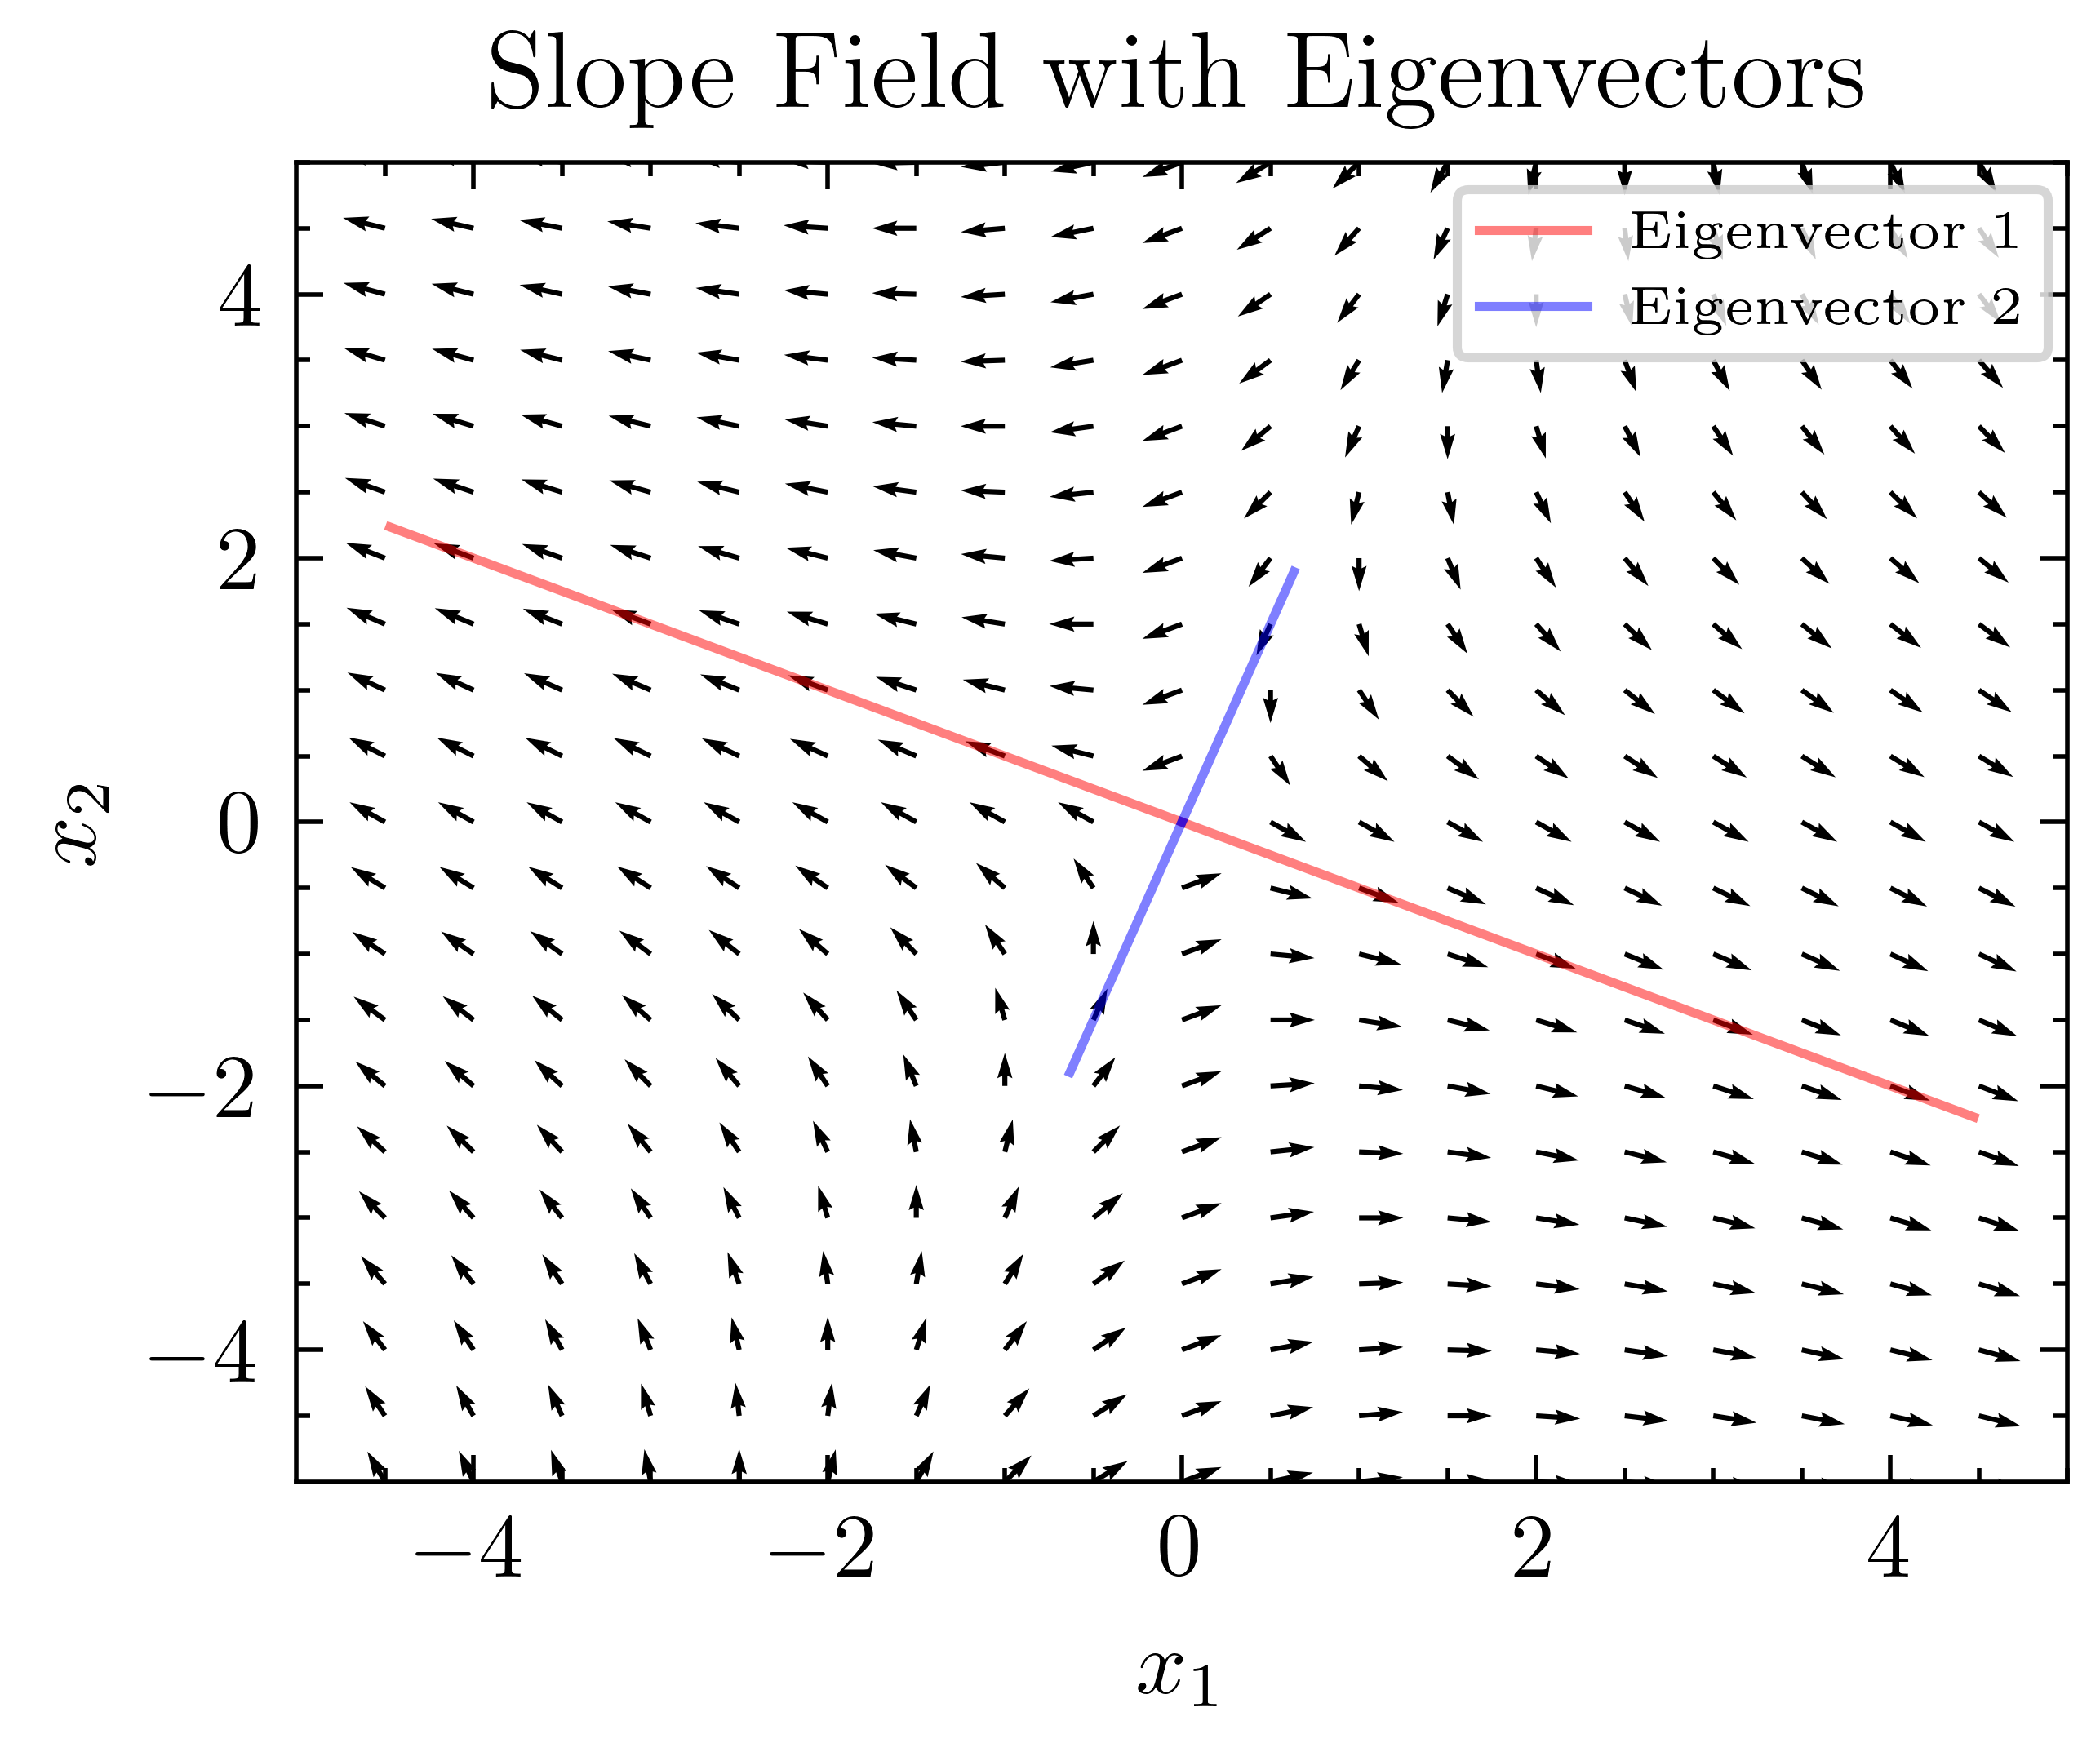
\includegraphics[scale=1.308]{slope-field.png}
\end{figure*}
\pagebreak

\subsection*{Problem 7} Find the power series solution centered at the ordinary point, $x_0=0$, for the following differential equation:

$$ y''-xy'=0.$$

Try it out before looking at the solution.
\pagebreak

\textbf{Solution to Problem 7:}

If all of the coefficients of our derivatives are analytic functions, then we can say that our solution will also be an analytic function. As such, it has a power series representation. We make the guess that that solution is of the following form:
$$ y_{\text{guess}} = \sum_{n=0}^{\infty} c_nx^n. $$
We take the derivatives of our guess to substitute into our differential equation and find a true statement.
$$ y_{\text{guess}}' = \sum_{n=1}^{\infty} (n)c_nx^{n-1}. $$
$$ y_{\text{guess}}'' = \sum_{n=2}^{\infty}(n-1)(n)c_nx^{n-2}.$$
Before any reindexing, we should be sure to make our substitution and distribute all factors:
$$ \left[\sum_{n=2}^{\infty}(n-1)(n)c_nx^{n-2}\right] - \underbrace{x}_{\text{distribute}}\left[\sum_{n=1}^{\infty}(n)c_nx^{n-1}\right] = 0 \quad\ldots $$
$$ \left[\sum_{n=2}^{\infty}(n-1)(n)c_nx^{n-2}\right] -\left[\sum_{n=1}^{\infty}(n)c_nx^{n}\right] = 0. $$
Now, we ask ourselves what is stopping us from combining these into one big sum and factoring out $x^{k}$? It's typically good convention to start off by ensuring all terms have a common factor of $x^{k}$. Let's do that with our first series.\\

Let $k=n-2$, implying that $n=k+2$:
$$ \left[\sum_{k=0}^{\infty}(k+1)(k+2)c_{k+2}x^{k}\right]\underbrace{ -\left[\sum_{k=1}^{\infty}(k)c_kx^{k}\right]}_{n=k} = 0. $$
Now that all series have a common factor of $x^{k}$, we can combine them, right? First, we need to make sure they start at the same index. They don't, so let's fix that:
$$ 2c_2 + \underbrace{\left[\sum_{k=1}^{\infty}(k+1)(k+2)c_{k+2}x^{k}\right]}_{\text{pulled out the 0th term}} -\left[\sum_{k=1}^{\infty}(k)c_kx^{k}\right] = 0. $$
Now, let's combine the three series into one big series, factoring out an $x^k$ in the process:
$$ 2c_2 + \sum_{k=1}^{\infty}\bigg[(k+1)(k+2)c_{k+2} - kc_k\bigg]x^k = 0. $$
The only way for this statement to be true is if:
$$ 2c_2= 0 $$
and
$$ (k+1)(k+2)c_{k+2} - kc_k = 0 $$
These two conditions are where we get our recurrence relations. The conventional form of a recurrence relation is to have the next term in the sequence to be equal to some combination of the previous terms. When we do this we get:
$$ c_2 = 0 \quad \text{ and }\quad c_{k+2} = \frac{kc_k}{(k+1)(k+2)}.  $$
With our recurrence relations, we can begin writing a few of the first coefficients in order to generalize a rule for the coefficients of our power series solution:
 $$ \begin{array}{rl}
k=1: & c_3 = \frac{1}{2\times 3} c_1\\

k=2: & c_4 = \frac{2}{3\times 4}c_2 \implies c_4=0 \\

k=3: & c_5 = \frac{3}{4\times5}c_3 \implies c_5 = \frac{1\times3}{2\times3\times4\times5} \\
k=4: & c_6 = \frac{4}{5\times6}c_4 \implies c_6 = 0 \\

k=5: & c_7 = \frac{5}{6\times7}c_5 \implies c_7 = \frac{1\times3\times5}{2\times3\times4\times5\times6\times7}
\end{array} $$

Now, if we look at the even terms:
$$
\begin{array}{rl}
p=1: & c_2 = 0\\
p=2: & c_4=0 \\
p=3: & c_6=0 
\end{array}
$$
Our rule for the even terms is simple:
$$ c_{2p} = 0. $$
Looking at the odd terms:
$$
\begin{array}{rl}
p=1: & c_3 = \frac{1}{2\times3}c_1\\
p=2: & c_5 = \frac{1\times3}{2\times3\times4\times5}c_1 \\
p=3: & c_7 = \frac{1\times3\times5}{2\times3\times4\times5\times6\times7}c_1
\end{array}
$$
We see an odd double factorial in the numerator, and a single factorial in the denominator. Using the dummy index, $p$, to describe this behavior, we have:
$$ c_{2p+1} = \frac{(2p-1)!!}{(2p+1)!}c_1. $$
With the coefficients for the even and odd terms of our solution, we have:
$$ y_e(x) = 0 $$
$$ y_o(x) = c_1\sum_{p=0}^{\infty}\frac{(2p-1)!!}{(2p+1)!}x^{2p+1}. $$
The full general solution is the superposition of the linearly independent solutions:
$$ y_g(x) = y_o + y_e $$
$$ y_g(x) = c_1\sum_{p=0}^{\infty}\frac{(2p-1)!!}{(2p+1)!}x^{2p+1}. $$
There is a problem here, however. Notice that we started off with a second order differential equation, which requires two arbitrary constants. $y_e$ being 0 messed that up for us, so we will add a constant to our general solution to ensure that it is in agreement with our expectations:

$$ \underline{\boxed{ y_g(x) = A +  c_1\sum_{p=0}^{\infty}\frac{(2p-1)!!}{(2p+1)!}x^{2p+1}}} $$
If we write out a few terms:
$$\underline{\boxed{y_g(x) = A + \underbrace{c_1x}_{(-1)!! = 1} + \frac{1}{6}c_1x^{3} + \frac{3}{120}c_1x^5 + \frac{15}{5040}c_1x^7 + \frac{105}{362880}c_1x^9 + \ldots}} $$
Wolfram Mathematica gives the solution:
$$ y(x) = \sqrt{\frac{\pi}{2}} c_1 \operatorname{erfi}\left(\frac{x}{\sqrt{2}}\right)+A. $$
How cool is it that we can find the solution to such a tricky differential equation. If you are curious to see what a plot of the first 100 terms of a specific solution looks like, I've included that below.

\begin{figure*}[ht!]
	\centering
	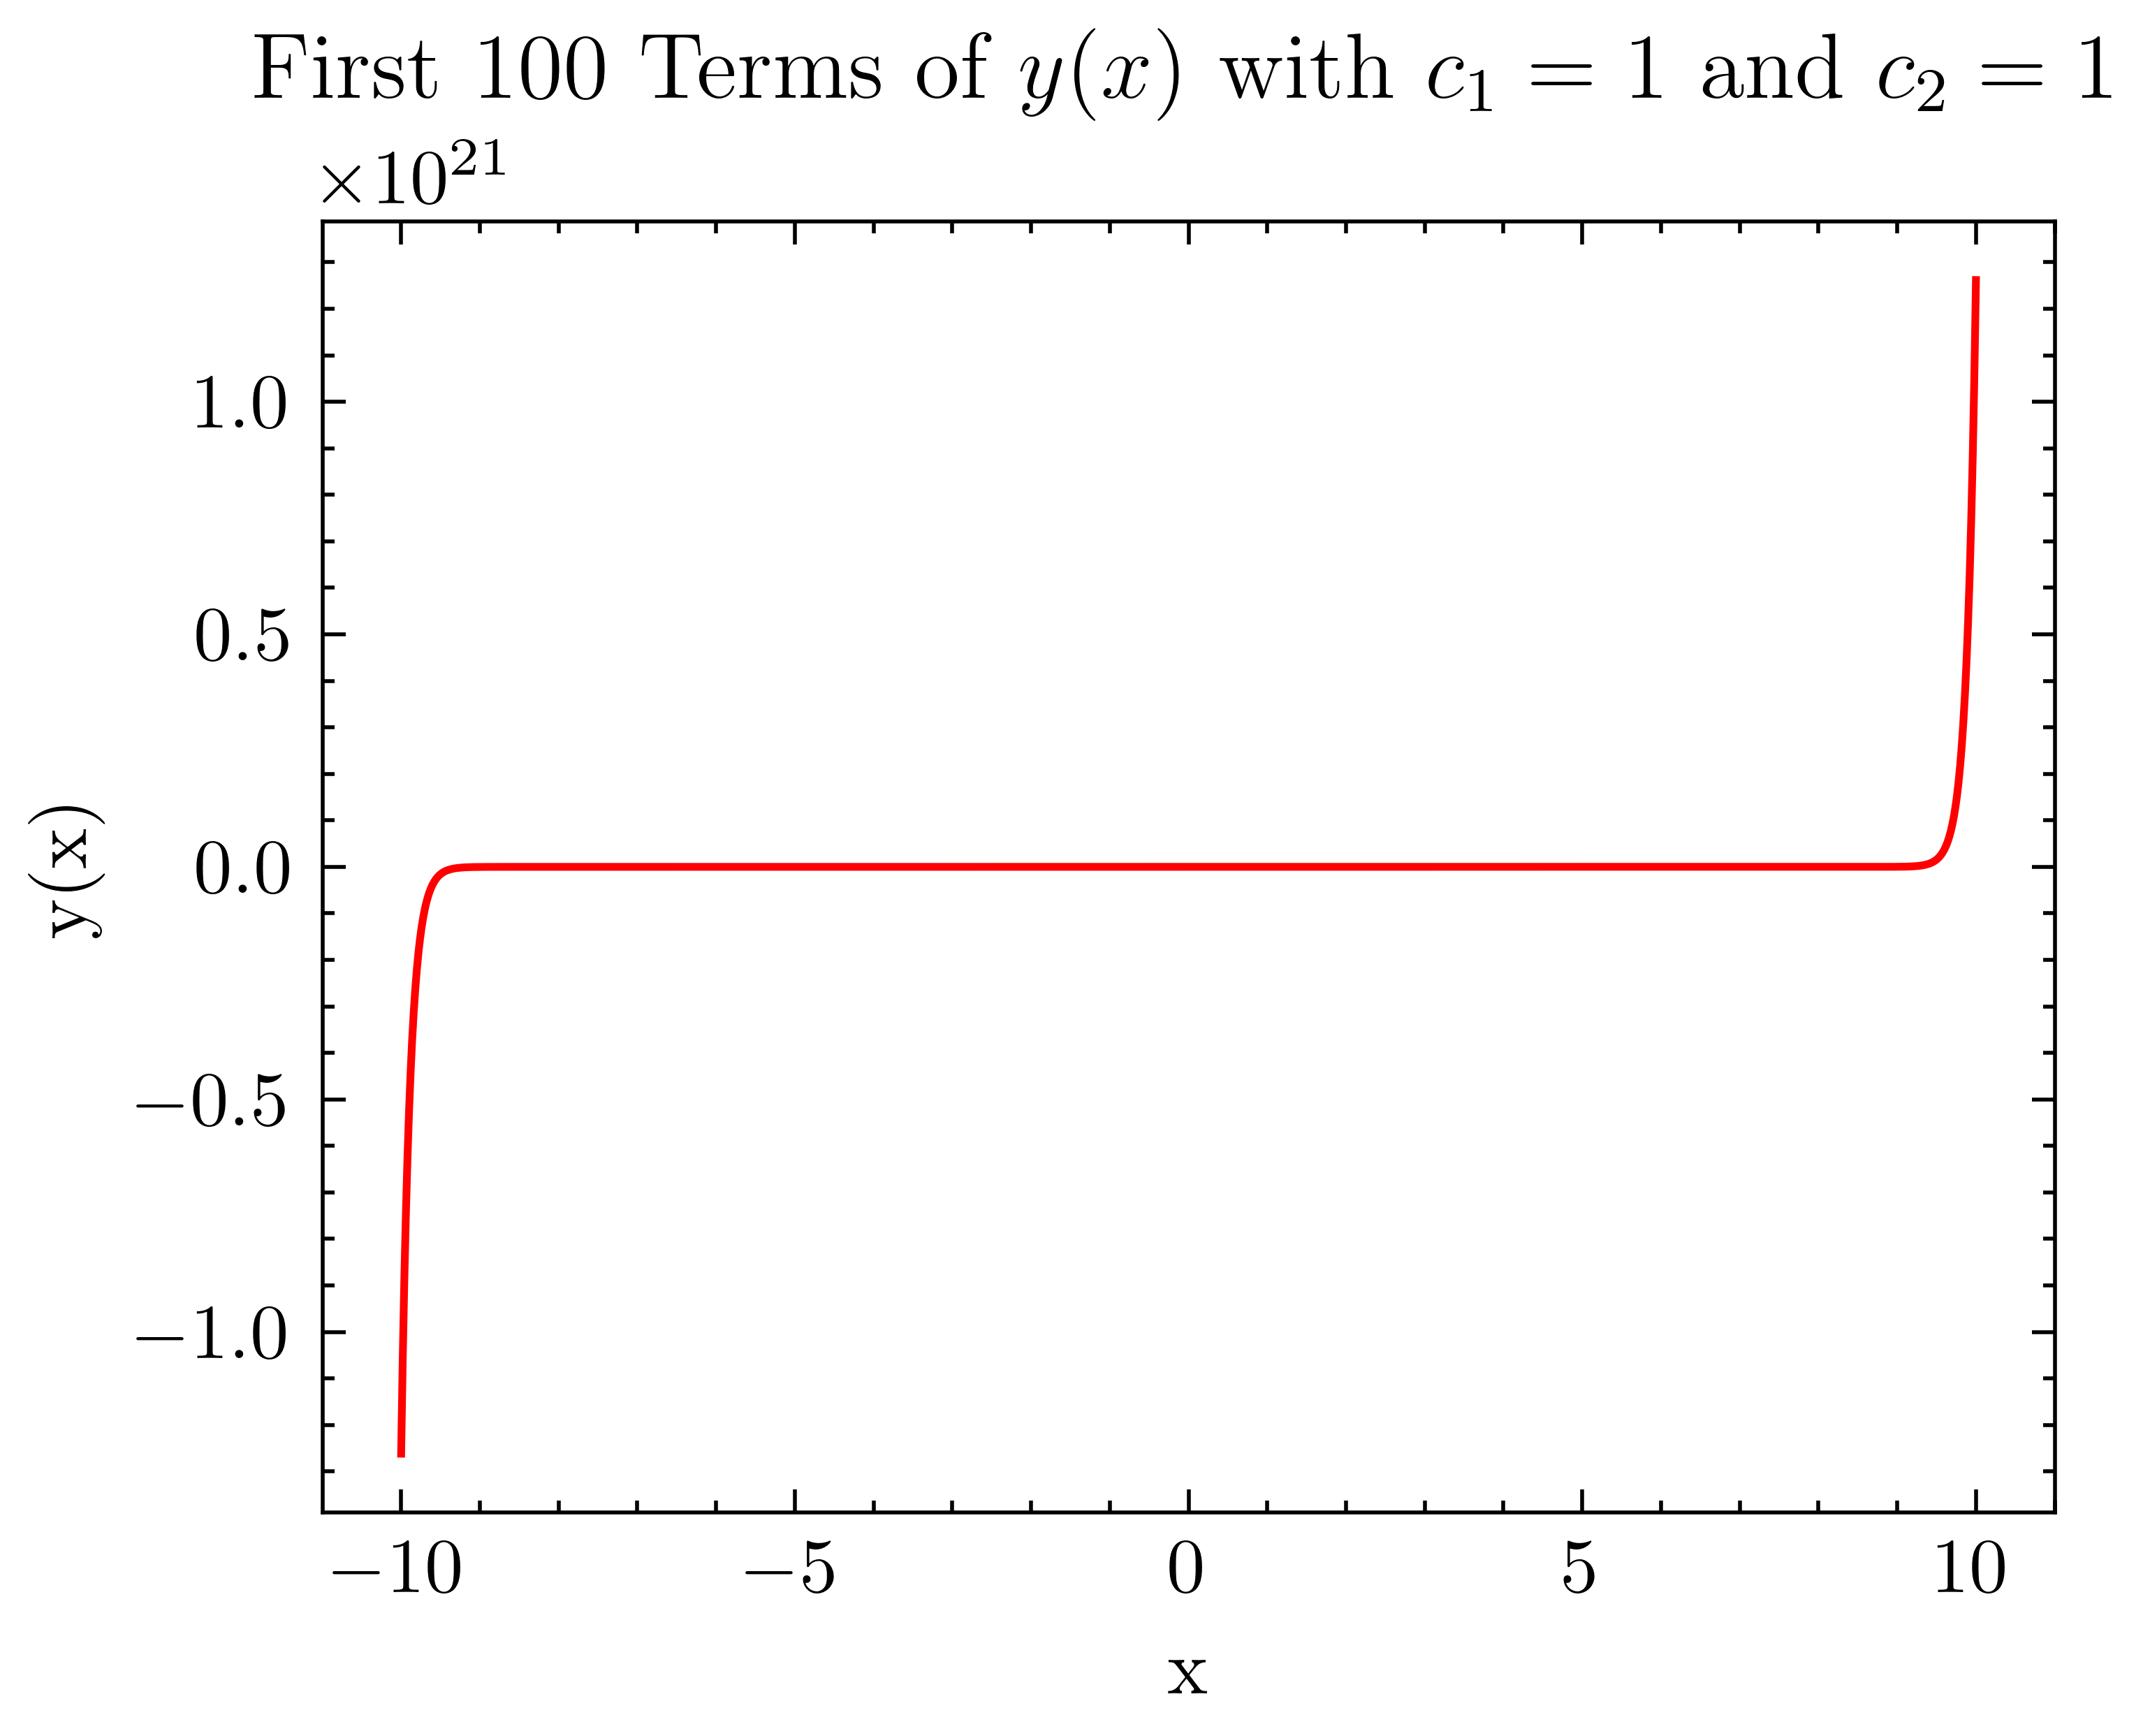
\includegraphics[scale=1.3]{last-one.png}
\end{figure*}

\pagebreak














\end{document}